%% Digital Systems
%% Continuous System Equivalence
\def\FileDate{10/01/21}
\def\FileVersion{1.0}
% ----------------------------------------------------------------
% Notes pages *********************************************************
% ----------------------------------------------------------------



\section*{Relationship between of $s$ and $z$}

Consider a simple function of time $f(t)=e^{-at}$, $t>0$. The Laplace transform of $f(t)$ is $F(s)=1/(s+a)$. This corresponds to a pole in the s-plane at $s=-a$. Now consider the sampled version of $f(t)$:
\begin{equation}
  \label{eq:l12e1}
  f(nT) = e^{-anT}
\end{equation}
where $f(nT)$ represents the value of $f(t)$ at the nth sampling instant $t=nT$ (T is the sampling period in seconds, the sampling frequency is $\omega_s=2\pi/T$ rad/s).
\begin{eqnarray}
	F(z) & = & \mathcal{Z}{e^{-anT}}=\sum_{n=0}^{\infty}e^{-anT}z^{-n}\\
	F(z) & = & 1+e^{-aT}z^{-1}+e^{-2aT}z^{-2}+e^{-3aT}z^{-3}+\cdots\\
	&=& \frac{1}{1-e^{-aT}z^{-1}} 	\label{eq:l12e2}
\end{eqnarray}
This result is summarised in \sref{slide:l12s1} and \sref{slide:l12s2}.
\begin{slide}\label{slide:l12s2}
  \heading{Mapping between between $s$ and $z$}
\begin{itemize}
  \item Generalising the previous result we can say that $s$ is related to $z$ by the mapping $z=e^{sT}.$
  \item Various properties of the z-plane follow from this `mapping'.
  \item s-plane stability boundary $s=j\omega$ maps to the unit circle $|z|=1$ in the z-plane.
  \item Maximum frequency is half the sampling frequency $\omega_s/2$ (a consequence of Nyquist's sampling theorem) and is mapped to the negative real axis in the z-plane.
\end{itemize}
\end{slide}

\begin{slide}\label{slide:l12s3}
  \heading{Stability in the z-plane}
\begin{itemize}
  \item Because the stability boundary is a unit circle, Routh-Hurwitz and Nyquist stability tests no longer work.
  \item The Jury test is a similar test to the Routh-Hurwitz test but it is more involved.
  \item The design curves for constant natural frequency $\omega_n$, damping ratio $\zeta$, $\sigma_d$ and $\omega_d$ are also distorted by the mapping.
  \item Use the Matlab function \emph{zgrid} to see the mapping.
\end{itemize}
\end{slide}

\begin{slide}\label{slide:l12s4}
  \heading{z-plane Design Curves}
  \begin{center}
    \scalebox{0.3}{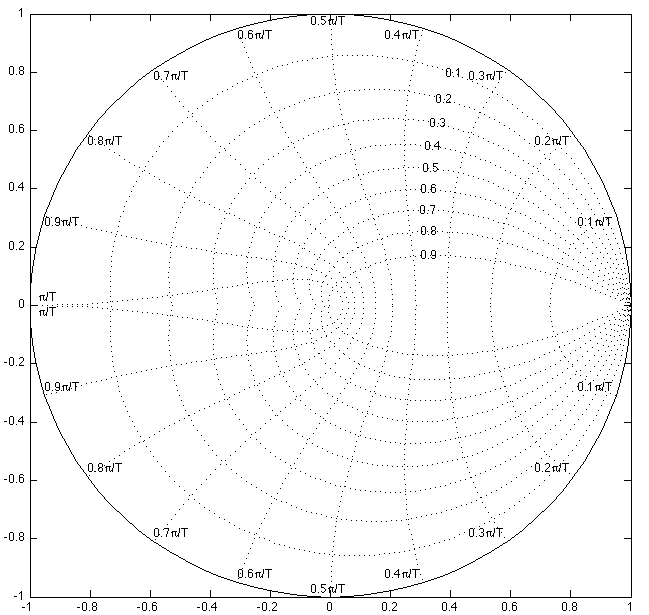
\includegraphics{pictures/zgrid.png}}
  \end{center}
\end{slide}


%----------------------------------------------------------------
% The end of notes
% ----------------------------------------------------------------
\endinput

% Local Variables:
% TeX-master: "lecture03"
% End:
